\chapter{基于半优化CycleGAN的非平行语料语音转换}

\section{引言}
上文介绍了非平行语料语音转换的基本概念及其常见方法,并详细介绍了基于CycleGAN的语音转换方法。
尽管这些方法极大地推动了非平行语料语音转换的技术发展,但是在目前的相关技术里转换语音的音质依旧存在较大的提升空间。

本章基于CycleGAN提出了一种改进的语音转换框架,该框架主要包含两个改进:半优化的CycleGAN模型 (Semi-optimized CycleGAN) 
和基频辅助特征;同时为了提升音质,该框架使用WaveNet声码器替代传统声码器,使用梅尔频谱特征代替传统的梅尔倒谱特征。
半优化CycleGAN主要特性为两个非一致更新的生成器,即在训练过程中,每个循环只有一个生成器被更新,另一个生成器只被用来生成中间特征。
经过对每个生成器的更新过程进行分析,在标准CycleGAN中,部分更新过程会导致生成器在计算损失时受到带有噪声标签的影响,
并且不同的更新过程之间存在互斥现象,从而导致转换模型性能的下降。半优化CycleGAN即通过去除该部分更新过程来提升模型性能。
参考近年语音合成和语音转换在声码器方面的研究,我们使用梅尔频谱作为声学特征,
来替代传统的梅尔倒谱系数、非周期信息和基频这三个特征,并使用基于梅尔频谱的WaveNet模型作为声码器。
为了克服CycleGAN模型对梅尔频谱中音调信息的学习能力不足的问题,提出在训练过程中使用基频特征作为梅尔频谱特征的辅助特征来共同训练,
该改进在保持使用梅尔频谱作为WaveNet的特征下,有效解决了转换音频中音调错误的问题。
本章将首先详细介绍基于梅尔频谱的WaveNet声码器在语音转换中的应用,然后阐述所提出的包含半优化CycleGAN和基频辅助特征的非平行语料语音转换系统,
最后对实验配置和实验结果进行说明和分析。

\section{基于梅尔频谱WaveNet的平行语料语音转换}
\subsection{WaveNet声码器}
如上文所述,WaveNet是一种自回归的概率生成模型,该模型可以通过历史音频样本点,直接预测当前样本点的分布,其模型结构如图~\ref{fig:wavenetarch}所示

\begin{figure}[!htp]
    \centering
    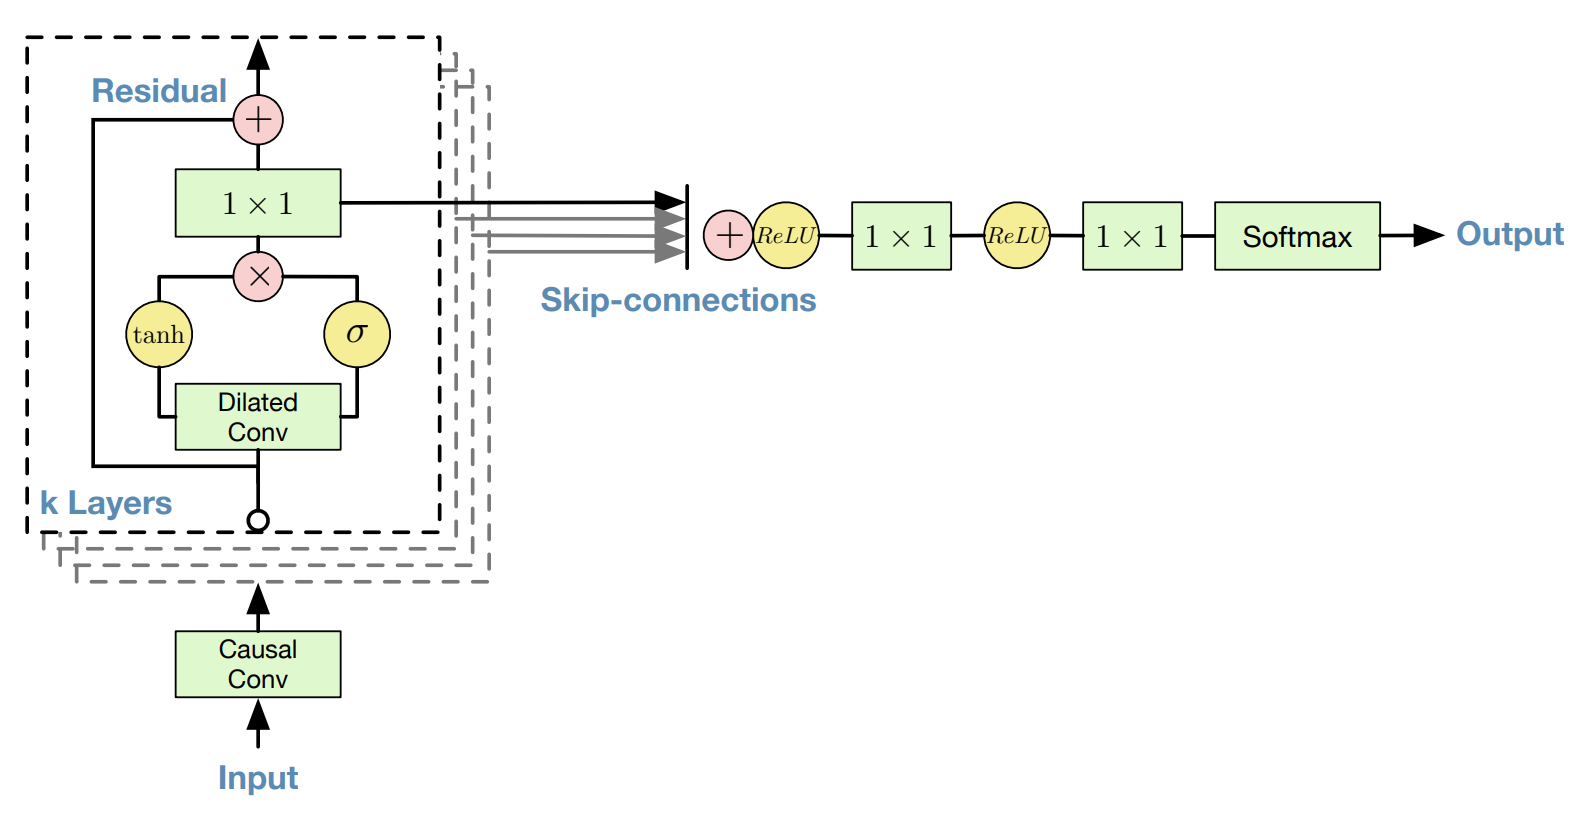
\includegraphics[width=12cm,trim=0 10 0 0,clip]{figure/4_wavenet.png}
    \bicaption[WaveNet模型结构图\cite{oord2016wavenet}]
    {WaveNet模型结构图}
    {Architecture of the WaveNet}
    \label{fig:wavenetarch}
\end{figure}

其中因果卷积 (Causal Conv) 和扩张卷积 (Dilated Conv) 可以有效增加模型的输入感受域。模型由多个跳跃连接模块构成,每个模块
包含一个扩张卷积和门控激励函数,其中的$1*1$代表卷积核大小为1x1的卷积网络。每个模块的输出可以表示为

\begin{equation}
    \mathbf{z} = tanh(W_{f,k} * \mathbf{x} + V^{T}_{f,k}\mathbf{h})\odot \sigma(W_{g,k} * \mathbf{x} + V^{T}_{g,k}\mathbf{h})
\end{equation}

其中$\mathbf{x}$和$\mathbf{z}$分别为输入和输出向量,$k$代表层编号,$f$和$g$分别代表门控激励函数中的滤波器和门,$W_{f,k}$,$W_{g,k}$,$V^T_{f,k}$,$V^T_{g,k}$
是可学习的权重矩阵,$*$是卷积操作,$\odot$是逐元素的乘法操作,$\sigma$是$sigmoid$函数,$h$表示全局条件向量。全局条件向量在WaveNet生成过程保持不变,常用于多说话人模型
中的说话人条件。对于局部特征来说,条件特征从单个向量变为了第二个特征序列$h_t$,该序列通常以帧为单位,因此采样率会低于音频信号,例如语音合成系统中的语义特征或者声码器中的声学特征。
通常会先将局部条件特征序列通过转置卷积或重复操作来将条件特征的采样率调整至与音频信号相同$\mathbf{y} = f(\mathbf{h})$,然后每一个模块的输出可变为

\begin{equation}
    \mathbf{z} = tanh(W_{f,k} * \mathbf{x} + V_{f,k} * \mathbf{y}) \odot \sigma (W_{g,k} * \mathbf{x} + V_{g,k} * \mathbf{y})
\end{equation}

此时$V_{f,k} * \mathbf{y}$和$V_{g,k} * \mathbf{y}$是一个1x1卷积层。整个网络的最终输出是一个$softmax$层,输出一个
256维度的概率向量。因为音频的采样点通常是浮点数,为了能够降低建模复杂度,需要首先用mu-law算法将浮点采样点分为256类,
将音频转换为一个256维的特征向量序列,具体公式如下

\begin{equation}
    f(x_t) = sign(x_t)\frac{ln(1+\mu \left| x_t\right|)}{ln(1+\mu)}
\end{equation}

其中$x_t$为t时刻的采样点,值域为$\left[-1,1\right]$ $sign$函数返回$x_t$的正负符号,$\mu$代表压缩的类别数,这里$\mu$取256。


\subsection{梅尔频谱特征转换}

\begin{figure}[!hbtp]
    \centering
    \bisubcaptionbox{传统语音转换}%
                    {Conventional Voice Conversion}%
                    [14cm]{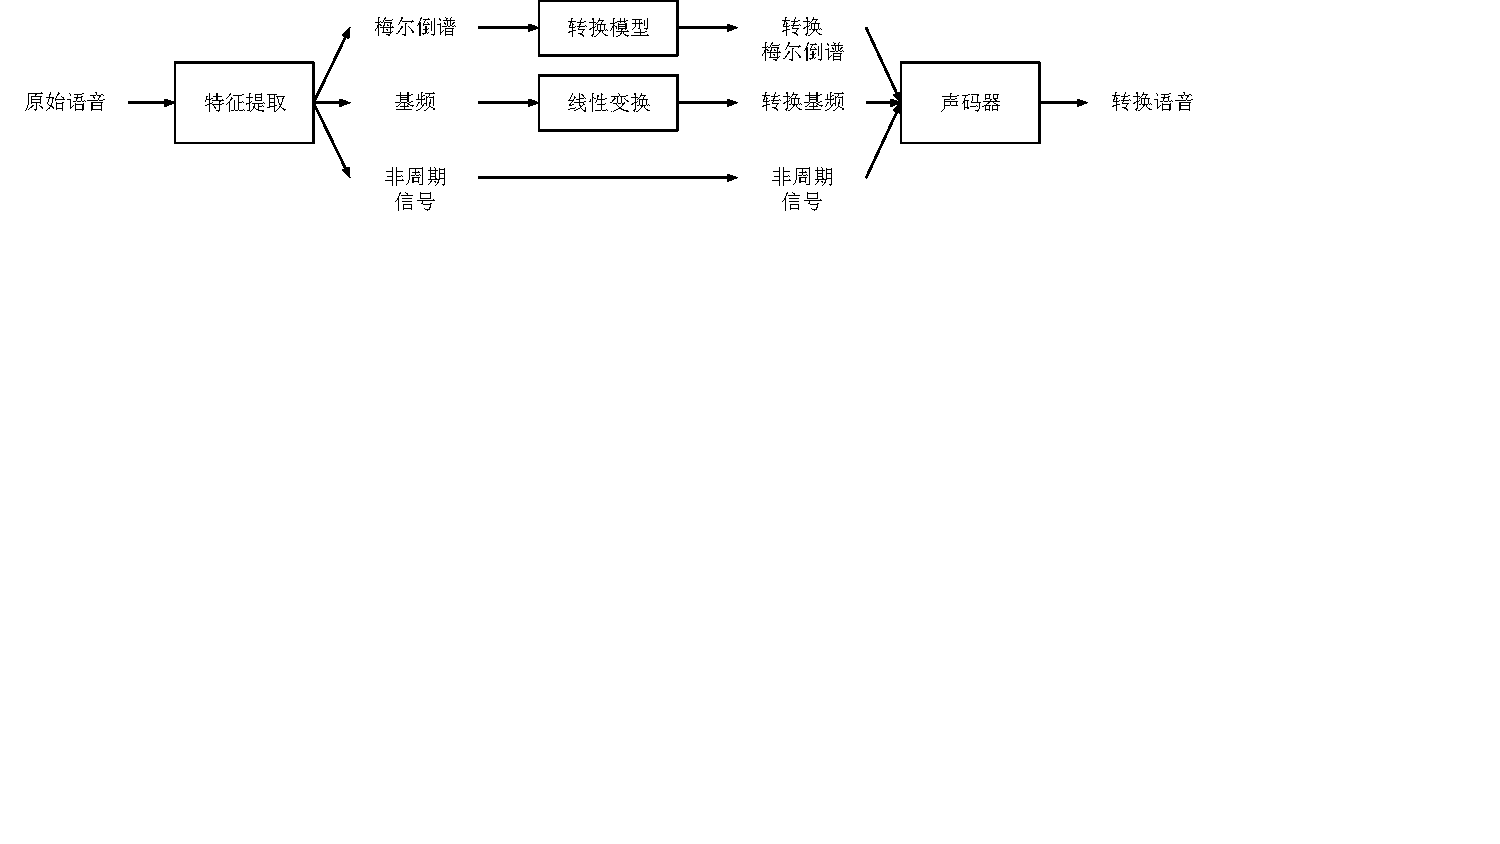
\includegraphics[width=14cm,trim=0 300 140 0,clip]{figure/4_vcmcep.pdf}} \\
    \vspace{0.5cm}
    \bisubcaptionbox{基于梅尔频谱的语音转换}%
                    {Mel-spectraogram based Voice Conversion}%bisubcaptionbox
                    [14cm]{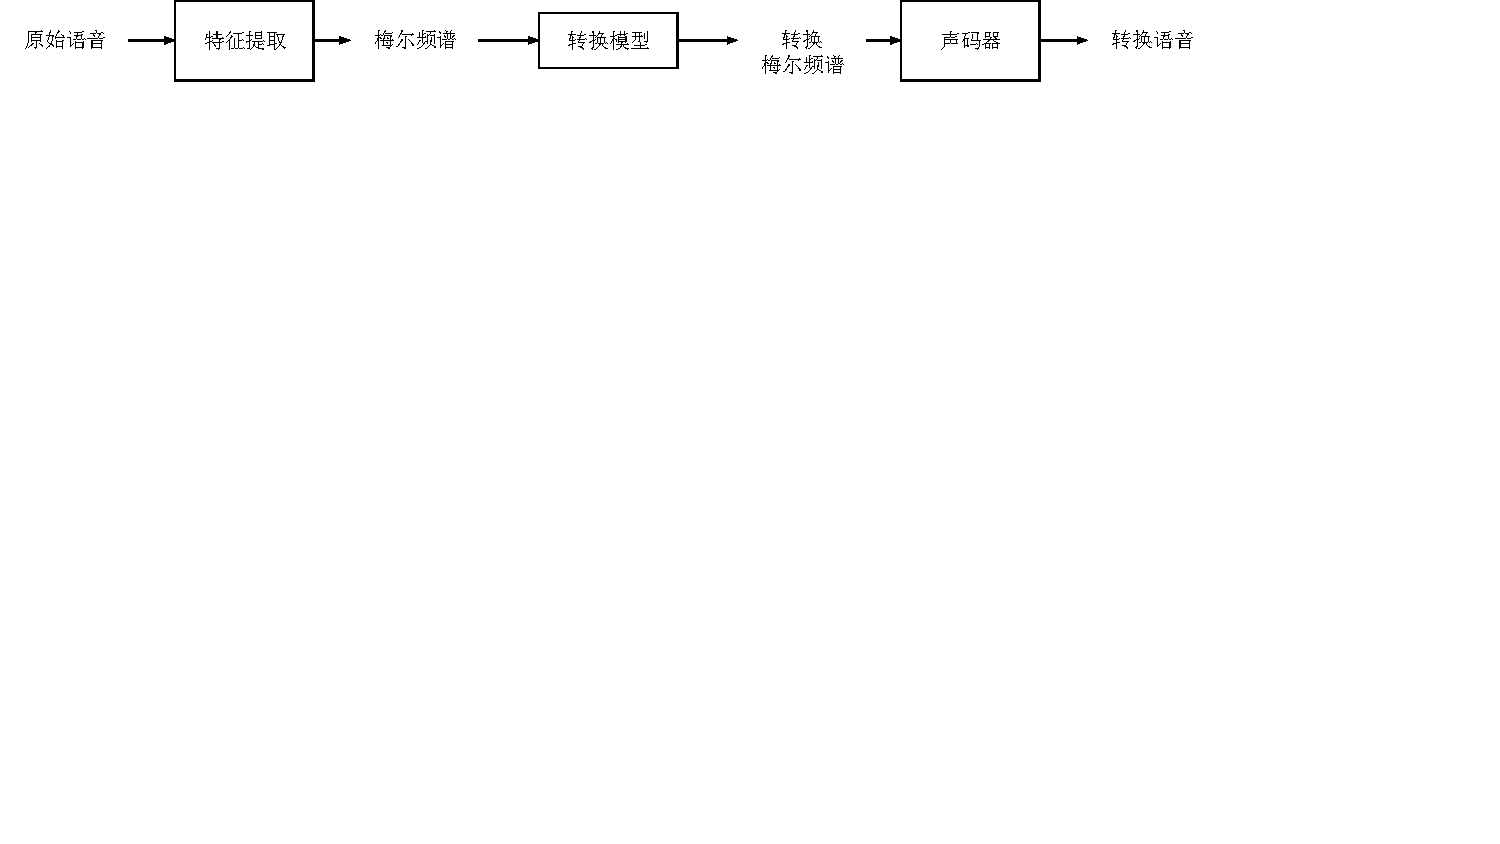
\includegraphics[width=14cm,trim=0 350 140 0,clip]{figure/4_vcmsp.pdf}}
    \bicaption{梅尔频谱语音转换和传统语音转换对比图}
              {Comparison of the Mel-spectrogram based Voice Conversion and the conventional Voice Conversion}
    \label{fig:vcdiff}
  \end{figure}

对于基于梅尔频谱的语音转换,可以使用任何转换模型将原始说话人的梅尔频谱特征转换为目标说话人,再通过WaveNet生成波形。
该方法与传统语音转换方法的区别如图~\ref{fig:vcdiff}所示,在传统的语音转换中,通过传统声码器会从语音中提取三个特征:梅尔倒谱系数 (Mgc) ,非周期信号 (bap) 和基频 (F0) 。
其中Mgc使用转换模型进行转换,bap保持不变,F0使用线性变换。
处理后的三个特征再通过数字信号声码器或神经网络声码器进行波形生成。
当使用梅尔频谱作为特征时,则直接从音频中提取梅尔频谱,然后将其作为转换特征进行训练和转换,声码器也直接从梅尔频谱中恢复波形。
梅尔频谱是将频谱映射到梅尔刻度 (Mel scale) 后取前$k$维得到的特征,梅尔刻度是基于彼此等距的听众对音高 (pitch) 的感性判断的刻度。

在\cite{chen2018high}中,作者在平行语料的语音转换任务中对比了
不同声学特征和声码器配置下转换语音的性能。
图~\ref{fig:wavenetworld4}为自然度主观意见分实验,其中bdl-slt和clb-slt分别为跨性别说话人组和同性别说话人组。在所示的
各组对照组中,N为自然音频,WNS为真实梅尔频谱特征的WaveNet合成音,WNC为真实梅尔倒谱特征的WaveNet合成音,WCS为转换
梅尔频谱的WaveNet合成音,WCC为转换梅尔倒谱特征的WaveNet合成音,MCC为转换梅尔倒谱特征的STRAIGHT合成音。可以看出
在梅尔倒谱特征中,STRAIGHT表现要优于WaveNet,但基于梅尔频谱的WaveNet不论在反合成还是在转换特征上合成,自然度都要好于
数字信号声码器。图~\ref{fig:wavenetworld1}和图~\ref{fig:wavenetworld2}展示了对转换语音相似度的偏好测试结果,可以看出不论是同性别还是跨性别上,
基于梅尔频谱的WaveNet (Msp WaveNet) 都要明显好于基于梅尔倒谱的WaveNet (Mcep WaveNet) 和STRAIGHT (Mcep STRAIGHT) 。


% \begin{figure}[!htp]
%     \centering
%     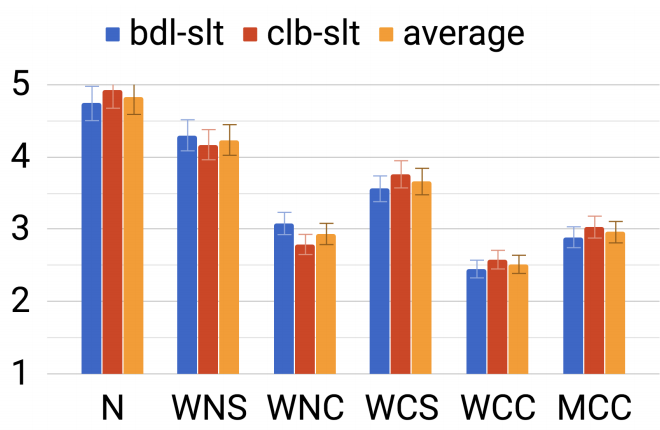
\includegraphics[width=10cm,trim=0 0 0 0,clip]{figure/4_wavenetworld4.png}
%     \bicaption[不同特征和声码器下转换语音的自然度对比\cite{chen2018high}]
%     {不同特征和声码器下转换语音的自然度对比}
%     {Comparison of converted speech naturalness on different features and vocoders}
%     \label{fig:wavenetworld4}
% \end{figure}

% \begin{figure}[!hbtp]
%     \centering

%     \bisubcaptionbox{相似度同性别}%
%                     {Intra-gender}%
%                     [10cm]{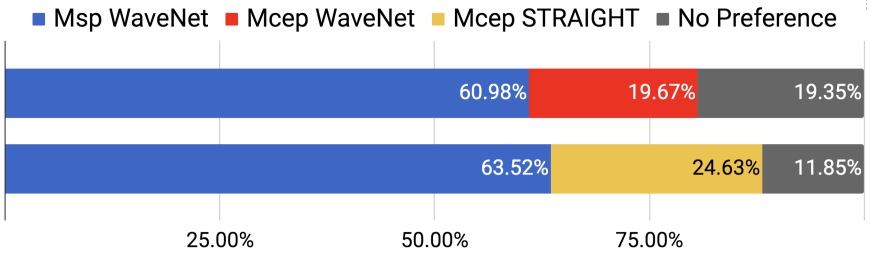
\includegraphics[width=10cm,trim=0 0 0 0,clip]{figure/4_wavenetworld1.png}} \\
%     \vspace{0.5cm}
%     \bisubcaptionbox{相似度跨性别}%
%                     {Inter-gender}%bisubcaptionbox
%                     [10cm]{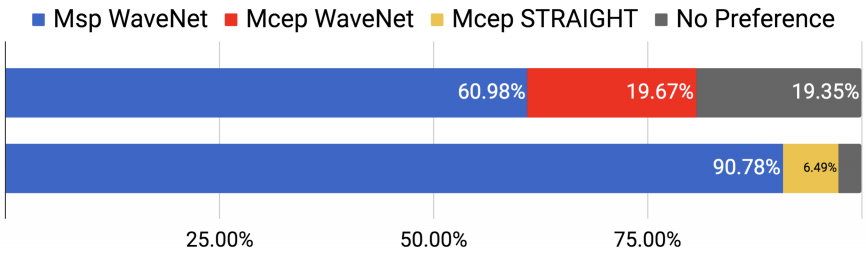
\includegraphics[width=10cm,trim=0 0 0 0,clip]{figure/4_wavenetworld2.png}}
%     \bicaption{不同特征和声码器下语音转换偏好测试对比图\cite{chen2018high}}
%               {Preference test on Voice Conversion of different features and vocoders}
%     \label{fig:wavenetworld1}
%   \end{figure}

\begin{figure}[!ht]
    \begin{subfigure}[b]{0.48\linewidth}
        %\rule{\linewidth}{1\linewidth}
        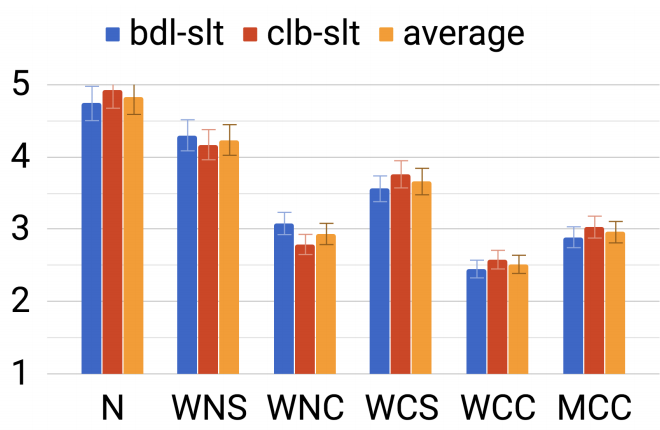
\includegraphics[width=\linewidth,trim=0 0 0 0,clip]{figure/4_wavenetworld4.png}

        \bicaption[MOS自然度]
        {MOS自然度}
        {Comparison of speech naturalness}
        \label{fig:wavenetworld4}
    \end{subfigure}
    \hfill
    \begin{minipage}[b]{0.5\linewidth}
        \begin{subfigure}[b]{\linewidth}
            %\rule{\linewidth}{0.5\linewidth}
            \centering
            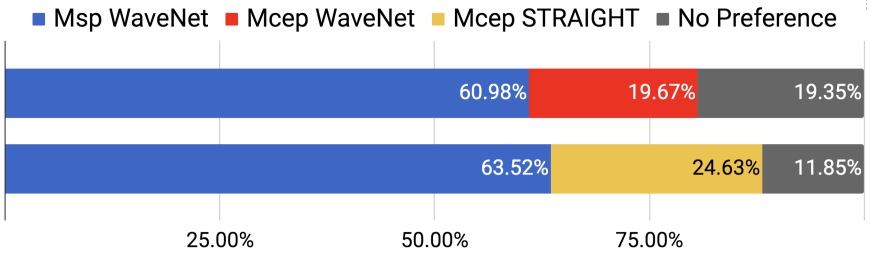
\includegraphics[width=0.8\linewidth,trim=0 0 0 0,clip]{figure/4_wavenetworld1.png}
            \bicaption[相似度同性别]{相似度同性别}{Intra-gender Similarity}
            \label{fig:wavenetworld1}
        \end{subfigure}\\
        \begin{subfigure}[b]{\linewidth}
            \centering
            %\rule{\linewidth}{0.5\linewidth}
            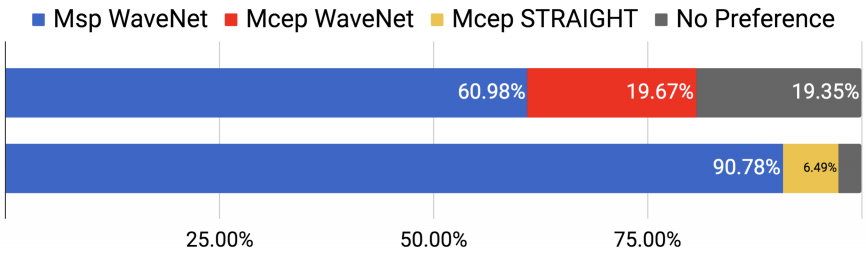
\includegraphics[width=0.8\linewidth,trim=0 0 0 0,clip]{figure/4_wavenetworld2.png}
            \bicaption[相似度跨性别]{相似度跨性别}{Inter-gender Similarity}
            \label{fig:wavenetworld2}
        \end{subfigure}
    \end{minipage}
    \bicaption{不同特征和声码器下语音转换对比图\cite{chen2018high}}
    {Comparison on Voice Conversion of different features and vocoders}
    \label{fig:wavenetworld}
\end{figure}

不同于梅尔倒谱,梅尔频谱不光包含了内容信息,还包含了音调信息,
相当于将传统的三个特征整合到了一起。因此,当使用梅尔频谱作为声学特征时,基频信息被隐性转换,
因此该转换会比线性转换拥有更复杂的音调转换能力,如前文所述,在平行语音转换中,先前的工作已经证明了在有监督的条件下,
梅尔频谱的音调转换能力要优于线性变换。但在无监督的条件下,由于没有真实标签,
同时CycleGAN的训练方式限制了生成器对局部信息的转换,导致模型较难从梅尔频谱中学习到基频表示。
因此基频的隐形转换拥有较大的难度。在我们的中文语音转换实验中,转换音频通常存在音调错误的问题,
尤其在男性转男性的实验中。我们提出使用基频辅助特征来提升模型的音调表示和转换能力,进而解决音调错误的问题。

\section{基于半优化CycleGAN的非平行语料语音转换系统}

\begin{figure}[!htp]
    \centering
    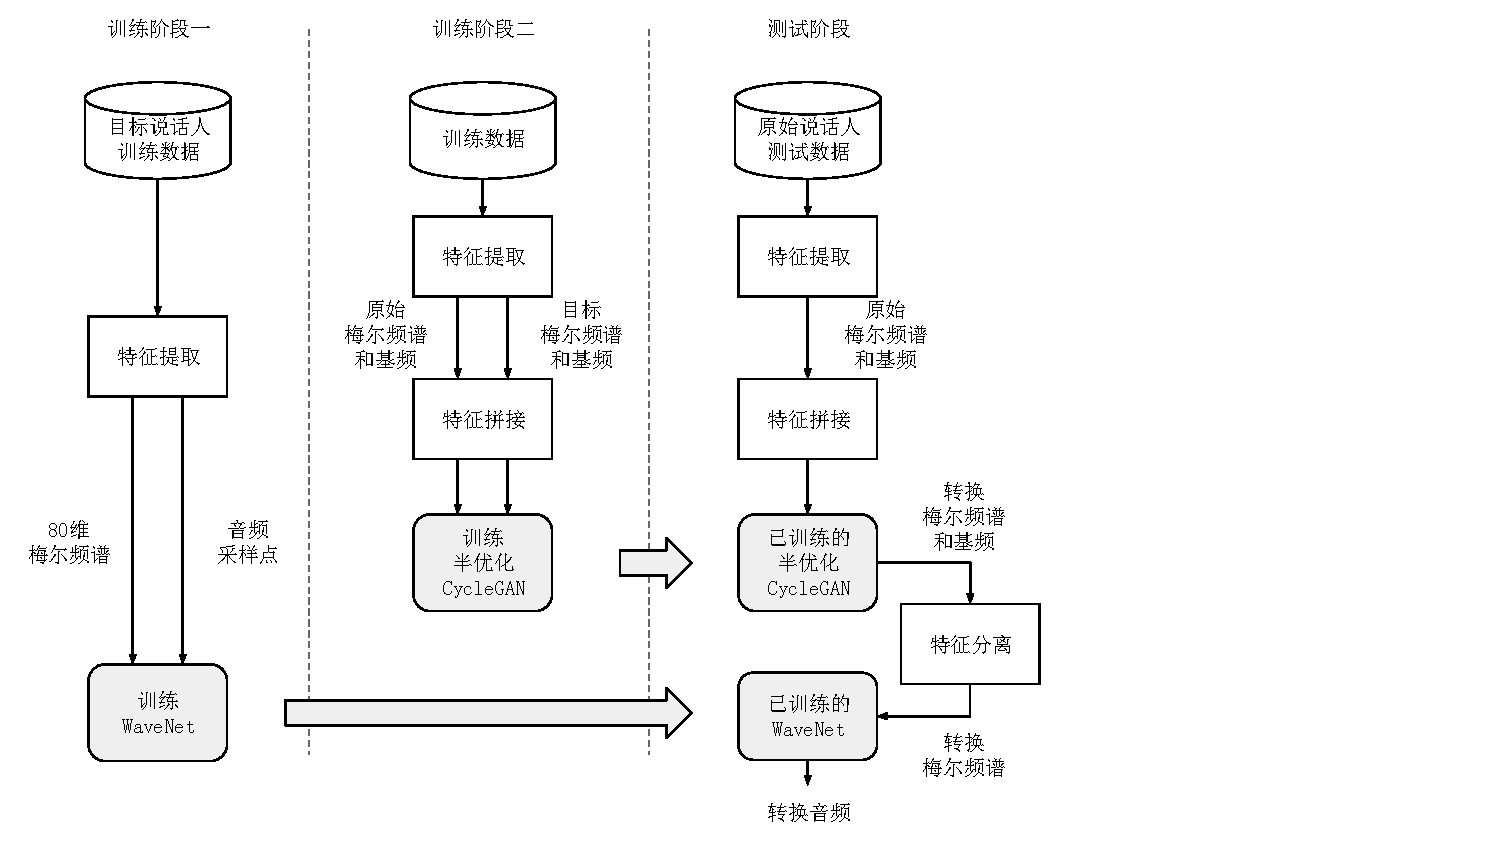
\includegraphics[width=12cm,trim=0 10 200 0,clip]{figure/4_proposedarch.pdf}
    \bicaption[基于半优化CycleGAN的语音转换系统结构图]
    {基于半优化CycleGAN的语音转换系统结构图}
    {Architecture of the semi-optimized CycleGAN based Voice Conversion}
    \label{fig:proposedarch}
\end{figure}

本文提出的改进框架,主要基于CycleGAN模型和基于梅尔频谱的语音转换,即:使用梅尔频谱作为声学特征,
CycleGAN作为语音转换模型,WaveNet作为神经网络声码器,以实现高音质的非平行语音转换。
结合上一节提出的现有框架的缺陷和不足,可以得出改进框架主要存在的两个挑战:
低音质的转换语音和非平行梅尔频谱转换中的发音错误问题。针对两个挑战,
本文分别提出半优化CycleGAN和基频辅助特征。在本节中,我们首先从最小更新过程的角度分析标准CycleGAN,
再介绍半优化CycleGAN。之后,再介绍使用基频辅助特征来解决音调转换错误的问题。

\subsection{半优化周期一致性生成对抗网络}

\begin{figure}[!htp]
    \centering
    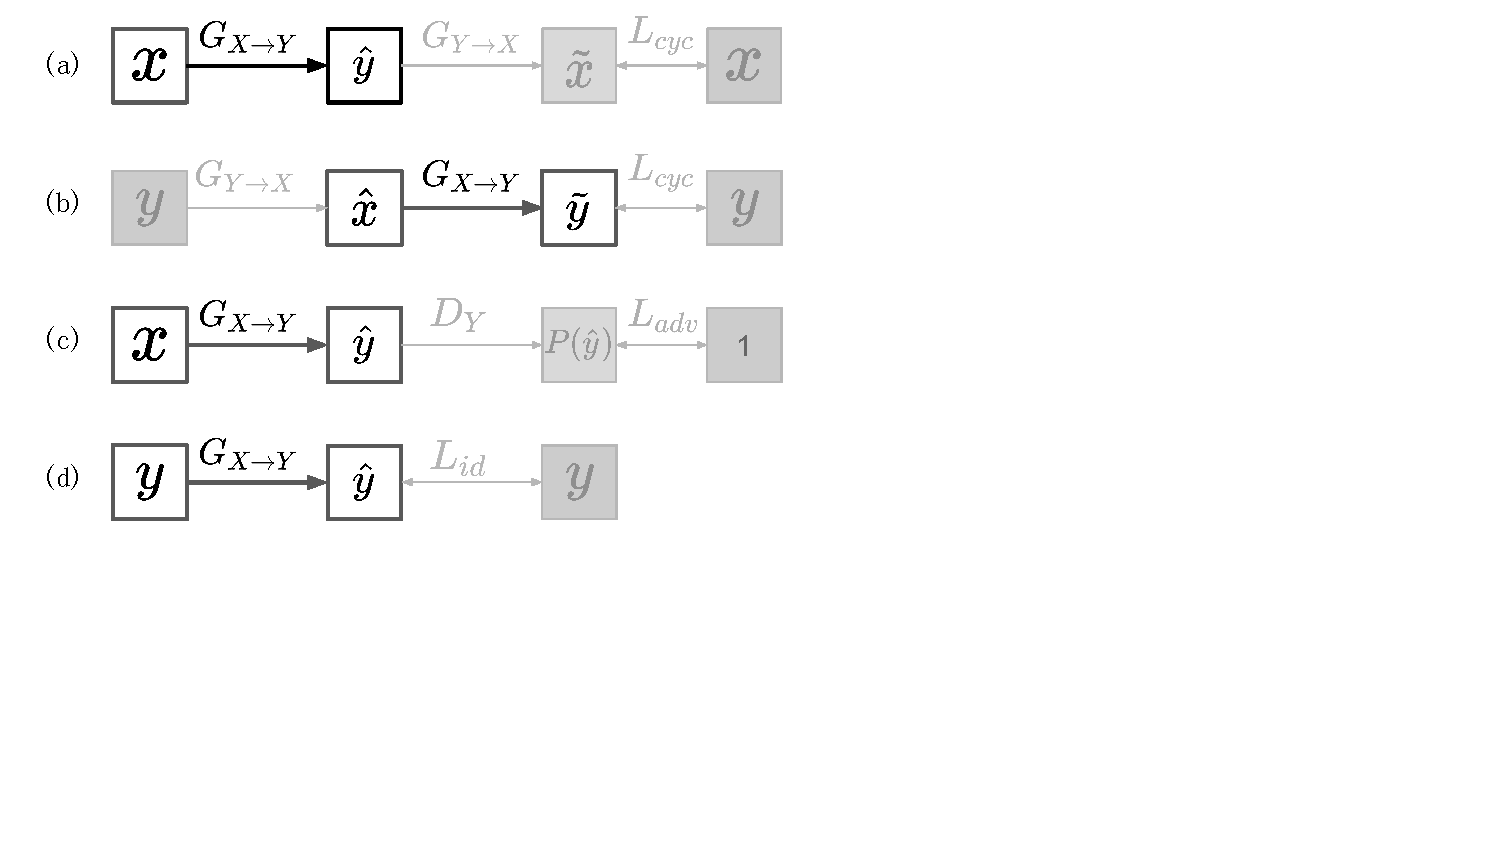
\includegraphics[width=8cm,trim=0 150 300 0,clip]{figure/4_dataflow.pdf}
    \bicaption[标准CycleGAN中最小更新过程示意图]
    {标准CycleGAN中最小更新过程示意图}
    {Schematic diagram of minimum update processes in conventional CycleGAN}
    \label{fig:dataflow}
\end{figure}

我们定义模型在训练过程中可以拆分的最小前向计算和反向梯度回传的过程作为一个最小更新过程。
从图~\ref{fig:dataflow}可以看出,对于每个生成器而言,一共有四个不同的最小更新过程来帮助模型训练,
其中(a)和(b)都来自于重构损失,(c)和(d)分别来自于对抗损失和身份损失。
这里我们只考虑单个生成器(以$G_{X\rightarrow Y}$为例)。
对每个最小更新过程进行分析,可以注意到对于(b)和(d),生成器的输出都有一个真实标签来计算损失。
然而对于(a)和(c),生成器是不存在一个真实的标签的,
并且其损失是由相连的下一个模型的梯度反传间接得到的。在(c)中,生成器和判别器对抗训练,
即当判别器尽可能去区分预测特征和真实特征时,生成器生成样本尽可能去欺骗判别器。
由于判别器本身在训练时存在样本和真实标签对,即真实特征和标签$1$。
因此通过对判别器输入预测特征,则可以得到预测特征和真实特征之间分布的误差。
该误差通过梯度反传至生成器的输出,则可以近似预测特征的损失,
使生成器的输出的数据分布更接近真实特征。然而,不同于(c),
(a)的下一个模型(即对偶的生成器$G_{Y\rightarrow X}$)并没有样本和真实标签对的训练数据,
因此经下一个模型反向传递的梯度无法保证能够很好地近似预测特征的损失;另一方面,
对偶的生成器在其身份损失的训练过程中(即更新过程(d)),
会输入和输出其目标特征,其反传的梯度会更接近于对偶生成器的目标特征分布,从而使得接近于,
这会影响当前模型训练,考虑到其可能带来的优点,更新过程(a)会对模型带来更多的负面影响。

\begin{figure}[!htp]
    \centering
    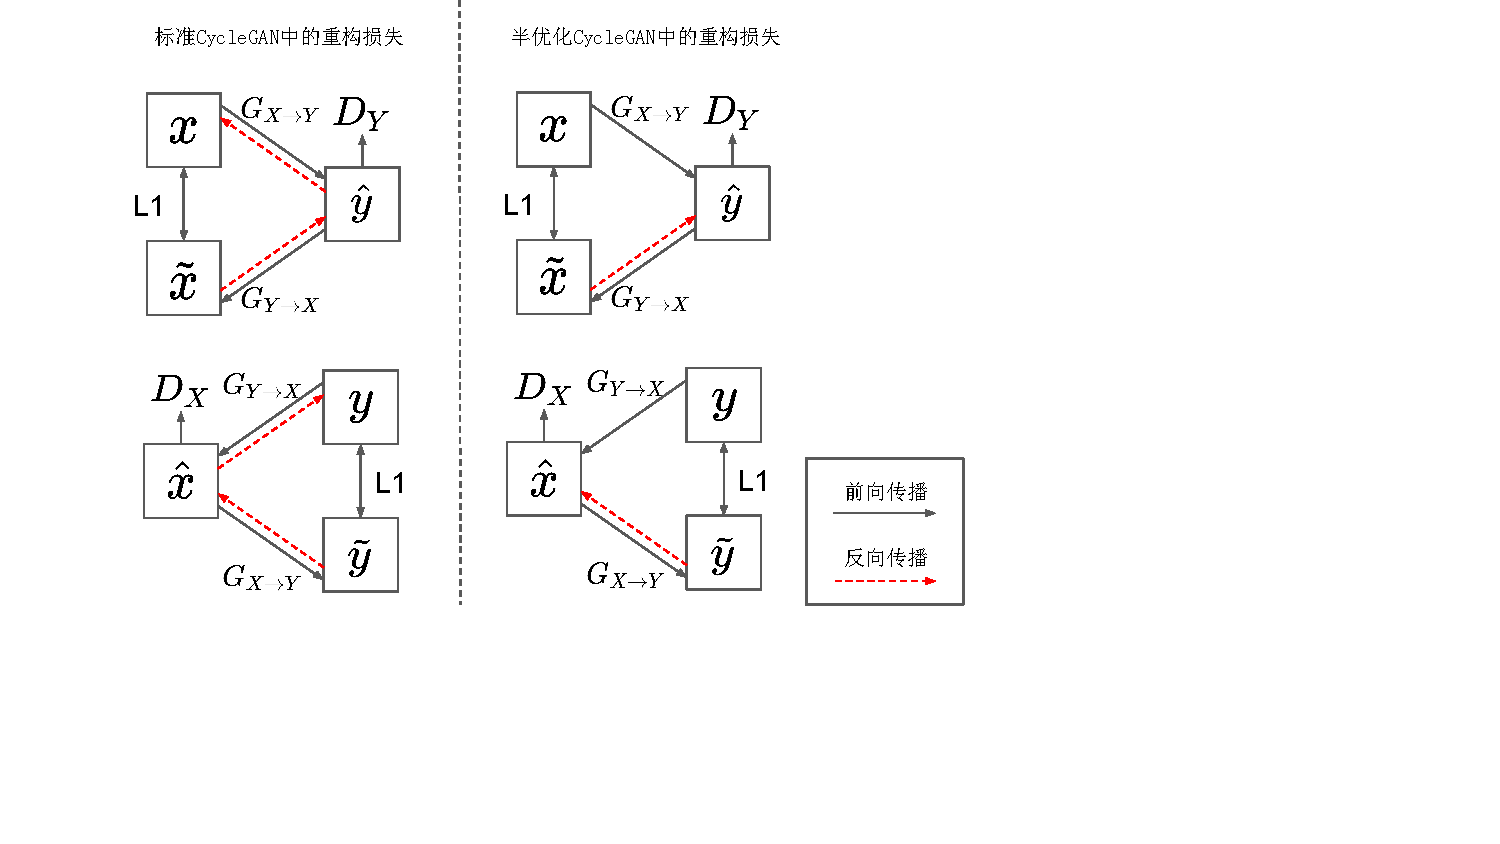
\includegraphics[width=10cm,trim=0 110 250 0,clip]{figure/4_semi.pdf}
    \bicaption[标准CycleGAN和半优化CycleGAN重构损失函数的对比图]
    {标准CycleGAN和半优化CycleGAN重构损失函数的对比图}
    {Comparison of Cycle-consistency loss between conventional CycleGAN and Semi-optimized CycleGAN}
    \label{fig:semi}
\end{figure}

因此我们对重构损失的训练策略进行了调整。如图~\ref{fig:semi}所示,我们去除了每个生成器的更新过程(a)。
因此对于每个循环,两个级联的生成器都会进行前向传播,但是只有第二个生成器会反向传播并更新,
此时第一个生成器只为第二个生成器生成带噪声的预测输入特征。我们称之为’半优化’。
重构损失公式变为

\begin{equation}
    L_{cyc}(G_{X\rightarrow Y},G_{Y\rightarrow X}) = L_{semicyc}(G_{X\rightarrow Y}) + L_{semicyc}(G_{Y\rightarrow X})
\end{equation}

其中

\begin{align}
    L_{semicyc}(G_{X\rightarrow Y}) & = \mathbb{E}_{y\sim P_{Data}(y)}\left[ \left| \left| G_{X\rightarrow Y}(G_{Y\rightarrow X}(y)) \right| \right|_1 \right] \\
    L_{semicyc}(G_{Y\rightarrow X}) & = \mathbb{E}_{x\sim P_{Data}(x)}\left[ \left| \left| G_{Y\rightarrow X}(G_{X\rightarrow Y}(x)) \right| \right|_1 \right]
\end{align}

在两次不同的循环中,分别只有一个生成器作为优化对象。
在实验中,我们发现半优化机制可以显著地减低噪声并提升转换语音自然度和说话人相似度。

\subsection{基频辅助特征}

我们使用梅尔频谱作为声学特征出于两个原因,一是其作为条件特征可以在WaveNet上生成相比梅尔倒谱和数字信号声码器更高音质的音频,
二是其本身包含了基频信息,因此可以使用神经网络进行更为复杂的基频隐性转换。然而如前文所述,
梅尔频谱直接作为CycleGAN的声学特征时存在发音错误的问题。主要原因分析如下。

如前文所述,
CycleGAN模型对说话人迁移的实现主要来自于对抗损失,其中判别器通过输入声学特征片段,
输出0到1之间的概率值来判断是否接近真实特征的分布。在经过大量的数据训练后,判别器能够对声学特征中的全局信息
(如说话人信息)有较强的判别能力,而随时间维度变化的局部信息(如语义,音调)在大量数据下很容易会被模型平均掉,
使模型对梅尔频谱中基频信息的表达学习较弱,从而导致转换特征存在发音错误的问题。理论上,如果加强判别器对序列建模的能力,如引入RNN,
可以使得模型对音调的判别能力增加,但这样做会使判别器对同为局部信息的语义的判别能力也会增加,而语义信息是希望模型进行平均的。
总的来说,发音错误的问题的改善需要通过不增加模型复杂度的前提下提升模型对梅尔频谱中基频信息表示的学习能力。
本章提出使用基频辅助特征来帮助模型更好地实现基频学习和转换。
如图~\ref{fig:proposedarch}所示,在训练阶段,梅尔频谱和基频特征被同时从原始音频和目标音频中提取。我们将两个特征拼接在一起,
并将其输入到生成器和判别器来同时训练。在测试阶段,两个特征被同时从原始音频中分析并转换,
但只有预测的梅尔频谱被用来作为条件特征进行波形生成。在实验中,基频辅助特征的引入有效地改善了合成音频中发音错误问题。

\section{实验分析}
\subsection{实验配置}

\begin{figure}[!htp]
    \centering
    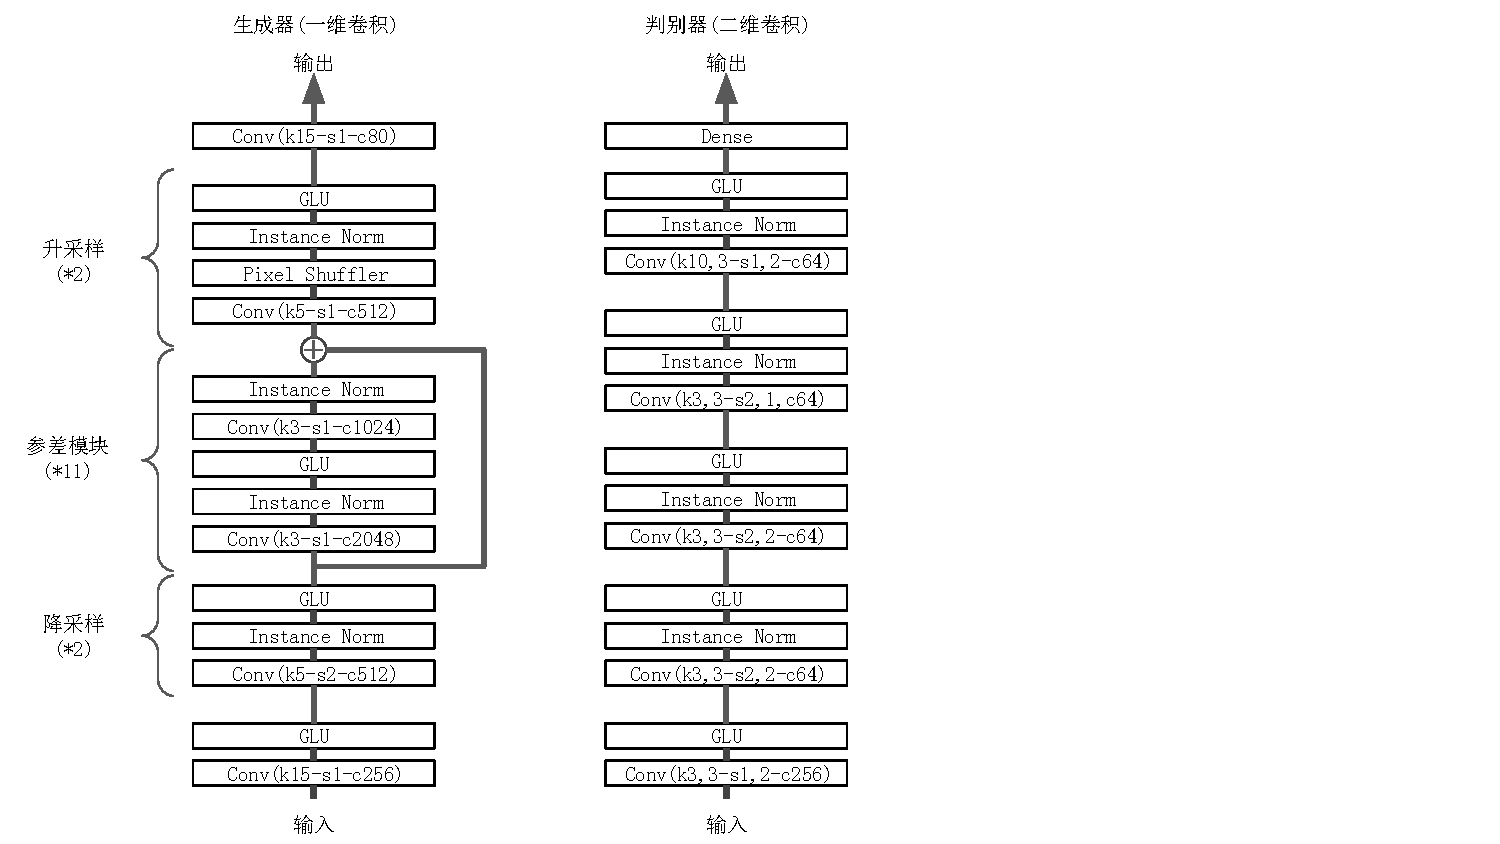
\includegraphics[width=12cm,trim=0 0 250 0,clip]{figure/4_networks.pdf}
    \bicaption[半优化CycleGAN网络结构图]
    {半优化CycleGAN网络结构图}
    {Architecture of the Semi-optimized CycleGAN}
    \label{fig:networks}
\end{figure}

我们在中文语音转换任务上评估了半优化CycleGAN和基频辅助特征的效果。所使用的中文数据集包含四个说话人,
两个男性说话人和两个女性说话人。所有训练和测试音频数据均录制于标准录音环境,且四个说话人都是以中文为母语的标准普通话说话人。
每个说话人的语音数据分为训练集、开发集和测试集,分别包含2000句,100句和20句,每句话音频长度在10s以内。
任意两个说话人的训练集数据均为非平行文本。音频采样率为16k。实验中特征首先通过WORLD声码器提取513维的频谱特征,513维的非周期信息和1维的基频特征,
之后用librosa\cite{mcfee2015librosa}和pysptk\cite{yamamoto2019r9y9}工具包提取80维的梅尔频谱特征和24维的梅尔倒谱特征。
帧移为5ms。注意到Tacotron2和平行语音转换任务中都使用了12.5ms帧移提取特征。然而在我们的实验中,
12.5ms的帧移会导致发音不完全或音素缺失的现象出现。我们因此使用5ms帧移来使用更细的频谱粒度来解决该问题。
虽然5ms的音质相比12.5ms相对较差,但是发音不完全的问题相比音质的下降更为严重。

首先使用每个说话人的训练数据各训练一个说话人相关的WaveNet声码器。其中WaveNet模型包含4个神经网络模块,
每个模块有6层神经网络。残差连接和门控层的隐层节点数为512,输出层的隐层节点数为256。
我们使用10个逻辑分布的混合逻辑分布来预测样本点分布。对于半优化CycleGAN,我们的模型结构如图~\ref{fig:networks}所示,
相比标准CycleGAN的网络结构,我们根据声学特征的帧移和维度对结构进行了调整:我们将生成器中残差模块的数量和卷积层的通道数乘2,
同时为了平衡生成器和判别器的对抗训练,判别器中四个降采样层的通道数都修改为64。
图中卷积层的标识k,s,c分别代表卷积核 (kernel) ,步长 (stride) 和频道数 (channel) 。生成器我们使用的是一维卷积,因为一维卷积
在抓取特征维度的总体关系的同时,更能够学习到特征的动态变化,因此在语音转换的任务中常使用一维卷积作为转换网络;然而在语音的后处理
任务 (Postfilter) 中,二维卷积更为常用,因为其更适合在改变特征形状的同时保留特征的原始结构,因此判别器使用二维卷积构建。
网络中Instance Normalization (IN) 是一种归一化方法,常用于风格迁移的任务中,其与常见的Batch Normalization (BN) 有所区别。
BN注重对每个batch进行归一化,保证数据的分布一致,因为判别模型中结果取决于数据的整体分布。但是在风格迁移的任务中,生成结果主要
依赖于具体的每个实例,所以对整体进行归一化并不适合用在风格迁移中,因此IN是对输入的高(Height)和宽(Width)进行归一化。由于IN的
训练和测试情况相同,不存在BN的不一致问题,因此也没有需要更新的参数。计算公式如下

\begin{equation}
    y_{bchw} = \frac{x_{bchw}-\mu_{bc}}{\sqrt{\sigma^2_{bc}+\epsilon}} * \gamma + \beta
\end{equation}

其中bchw分别代表特征的四个维度:batch,channel,height,width。$x$和$y$分别为输入和输出。$\gamma$和$\beta$是超参数。
$\mu_{bc}$和$\sigma^2_{bc}$计算方式如下

\begin{align}
    \mu_{bc} & = \frac{1}{HW}\sum^W_{w=1}\sum^H_{h=1}x_{bchw} \\
    \sigma^2_{bc} & = \frac{1}{HW}\sum^W_{w=1}\sum^H_{h=1}(x_{bchw}-\mu_{bc})^2
\end{align}

Pixel Shuffler是一种卷积网络中的升采样方法,其通过对特征矩阵进行变换和转置操作,将特征图的形状由$(B,f_1 * f_2 * C,H,W)$
转变为$(B,C,f_1 *H,f_2 *W)$。

数据载入部分我们使用了与CycleGAN-VC相同的策略,即在训练数据中随机截取连续128帧的特征片段。
所有网络都使用Adam优化器进行训练。训练batch大小设置为4。生成器和判别器的初始学习率分别为0.01和0.005,
不使用任何学习率调节策略。模型共训练350k步,身份损失只参与训练开始的前10k步。同时为了增强模型的鲁棒性,
在预测时,会将原始声学特征序列拆分为重叠的128帧片段,然后依次输入生成器,将生成的每个片段的中间部分提取出来,将他们拼接成最终的转换特征序列。

\subsection{客观评测}
本文首先采用梅尔频谱距离 (Mel-spectrogram Distorsion, Msd) 来判断转换模型在测试集上对特征转换的接近程度。
由于CycleGAN对抗学习的特性,其训练过程往往是不稳定的,模型性能与训练时长并不成正比关系。
因此我们记录了训练阶段模型在测试集上的梅尔频谱距离,频谱距离的计算使用了平行的测试数据,
这些数据不会参与模型训练。计算距离前会先用DTW算法对特征序列长度进行对齐。
我们在跨性别实验上对比了半优化CycleGAN和标准CycleGAN。实验结果如图~\ref{fig:msd}所示。
我们可以发现半优化CycleGAN所转换的梅尔频谱更接近目标特征,并且半优化CycleGAN的收敛曲线更为平稳。在实际实验中,
半优化CycleGAN也更容易训练和优化。

\begin{figure}[!hbtp]
    \centering
    \bisubcaptionbox{男性说话人转女性说话人}%
                    {Male to female}%
                    [12cm]{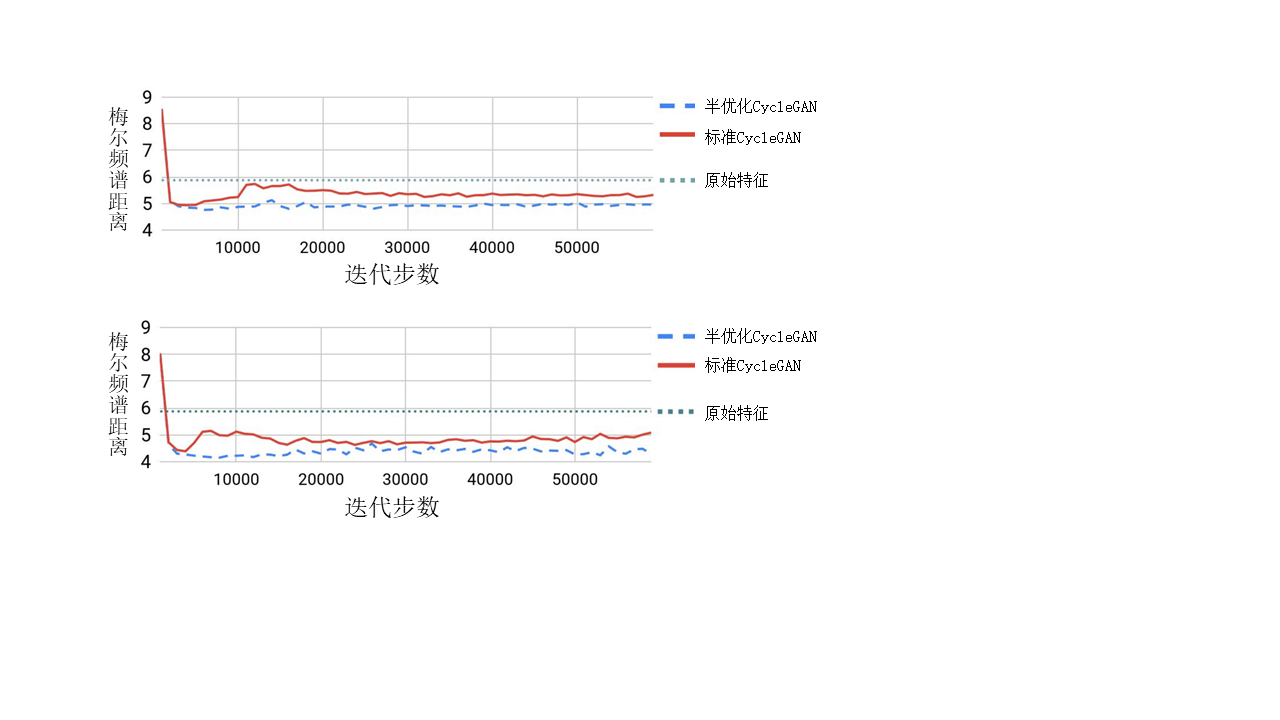
\includegraphics[width=12cm,trim=50 320 350 60,clip]{figure/4_msd.png}} \\
    \vspace{0.5cm}
    \bisubcaptionbox{女性说话人转男性说话人}%
                    {Female to male}%bisubcaptionbox
                    [12cm]{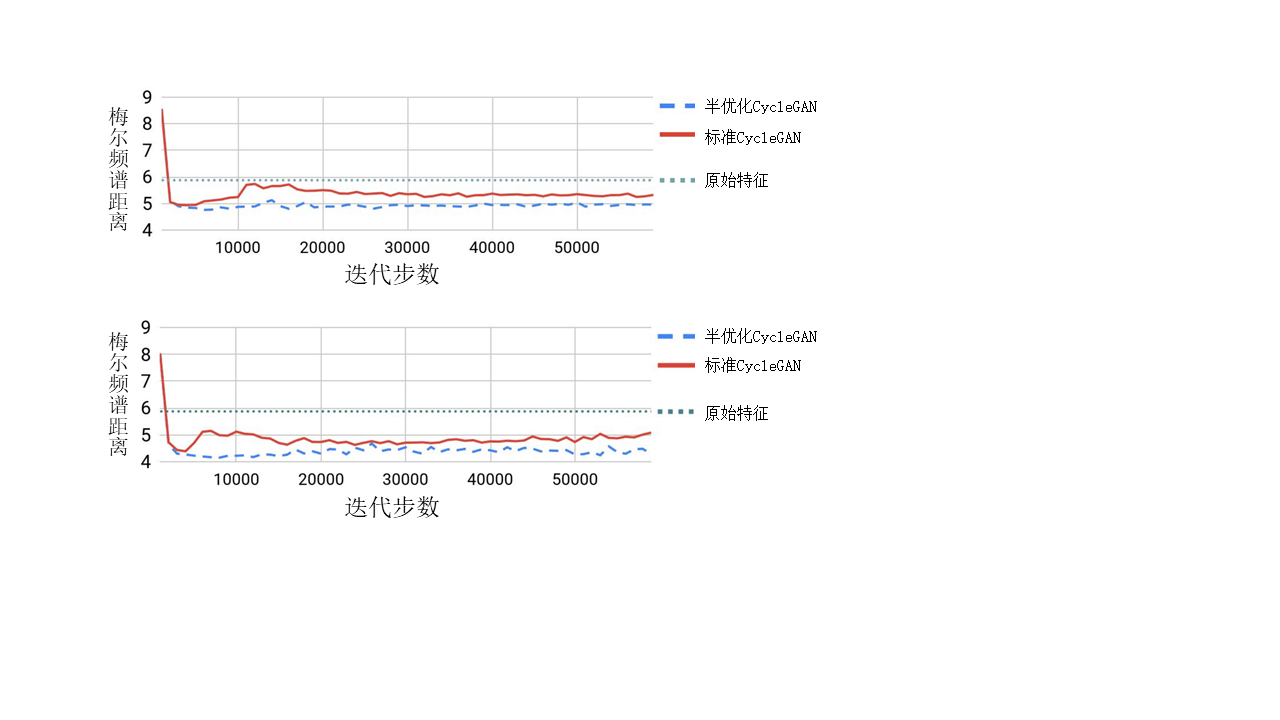
\includegraphics[width=12cm,trim=50 150 350 240,clip]{figure/4_msd.png}}
    \bicaption{标准CycleGAN和半优化CycleGAN在训练过程中梅尔频谱距离的对比}
              {Comparison of Msp distance between conventional CycleGAN and SoCycleGAN during training}
    \label{fig:msd}
  \end{figure}

为了验证基频转换的效果,在平行测试集上分别用WORLD声码器从转换音频和目标音频中提取基频特征,
统计各自的基频分布以及对齐后的标准误差。如表~\ref{tab:mse}所示,其中Source,Target分别代表原始真实特征
和目标真实特征,Linear代表线性变换的基频特征,Proposed w/o LF0代表没有使用基频辅助特征转换的基频,
Proposed代表使用了基频辅助特征后转换的基频。可以发现相比于线性变换,
基频辅助特征所转换的基频误差有较为明显的降低,同时基频分布也较接近目标的基频分布。
我们认为这是因为:(1)梅尔频谱可以实现基频的隐式转换,从而可以对基频进行比线性变换更复杂的变换映射;
(2)辅助特征通过引入显示的基频特征,可以帮助模型学习梅尔频谱中和基频信息高度相关的隐含表示,
进而提升基频的转换能力。

\begin{table} 
    \centering 
    \bicaption{转换基频和目标基频之间误差、均值和方差的对比}{Comparison of MSE, mean and standard deviation between target and converted F0}

    \begin{subtable}[t]{0.9\textwidth}
        \centering
        \bicaption{女性说话人转男性说话人}{Female to male}
        \begin{tabular}[t]{ cccc }
            \toprule
            % \hline
            %\multirow{1}{*}{Methods} & \multicolumn{3}{|c|}{Female to male} \\
             %\cline{2-4}
            Methods  & RMSE (Hz) & Mean (Hz) & Std (Hz) \\
             %\hline
             %\hline
            \midrule
            Target                  & 0 & 133.25 & 34.72             \\
            \midrule
            %\hline
            %\hline
            Source                    & 65.12 & 236.11 & 55.00            \\
            %\hline
            Linear                       & 17.13 & 127.10 & 28.58               \\
            %\hline
            Proposed w/o LF0                       & 17.44 & 124.66 & 27.74            \\
            %\hline
            Proposed                       & \textbf{16.69} & 126.31 & \textbf{29.82}   \\
            %\hline
            \bottomrule
            \end{tabular} 
        \label{tab:f0f2m}
    \end{subtable}
    \bigskip
    \vspace{1mm}
    \quad
    \begin{subtable}[t]{0.9\textwidth}
        \centering
        \bicaption{男性说话人转女性说话人}{Male to female}
        \begin{tabular}[t]{ cccc }
            \toprule
            %\hline
            %\multirow{2}*{Methods} & \multicolumn{3}{|c|}{Male to female}\\
             %\cline{2-4}
             Methods & RMSE(Hz) & Mean (Hz) & Std (Hz) \\
             %\hline
             %\hline
            \midrule
            Target                   & 0 & 236.11 & 55.00            \\
            \midrule
            %\hline
            %\hline
            Source                        & 67.10 & 133.25 & 34.72            \\
            %\hline
            Linear                     & 34.13 & 248.04 & 67.04              \\
            %\hline
            Proposed w/o LF0                   & 32.51 & 254.71 & 59.53              \\
            %\hline
            Proposed                      & \textbf{30.37} & 248.66 & \textbf{58.92}   \\
            %\hline
            \bottomrule
          \end{tabular}
        \label{tab:f0m2f}
    \end{subtable}

\label{tab:mse}
\end{table}  

\subsection{主观评测}
为了对系统的转换效果进行测试,我们采用较为普遍的主观听音测试来评测转换语音的质量。
所有的听音测试在同性别和跨性别上都进行了测试,并从测试集中随机选择了十句话让测试人员评测。
每一句话在每一次测试中被至少六个测试人员评价。不同系统的转换音频以随机顺序提供给测试人。
测试人皆是以普通话为母语的说话人。为了验证所提框架和改进的有效性,
我们使用模型消融测试 (Ablation test) 来比较不同系统。所比较的系统实验配置如下:

\begin{enumerate}
    \item N:真实语音
    \item Re:真实语音提取的梅尔频谱特征,用WaveNet合成
    \item B:标准CycleGAN预测的梅尔倒谱系数特征,用WORLD合成(基线系统,baseline)
    \item P:半优化CycleGAN预测的梅尔频谱特征,引入基频辅助特征,用WaveNet合成
    \item P w/o SoCycleGAN:标准CycleGAN预测的梅尔频谱特征,引入基频辅助特征,用WaveNet合成
    \item P w/o F0:半优化CycleGAN预测的梅尔频谱特征,无基频辅助特征,用WaveNet合成
\end{enumerate}

为了评测自然度,我们使用平均主观意见分 (Mean Opinion Score, MOS) 测试。
系统N和Re分别作为语音音质的上限分数和声码器的上限分数。
除此之外我们也测试了所提出的系统在小数据集上的表现,即在相同配置下100、200、500句话训练集的效果。
为了评测相似度,我们使用相同/不相同测试 (same/different test) 。

\begin{figure}[!htp]
    \centering
    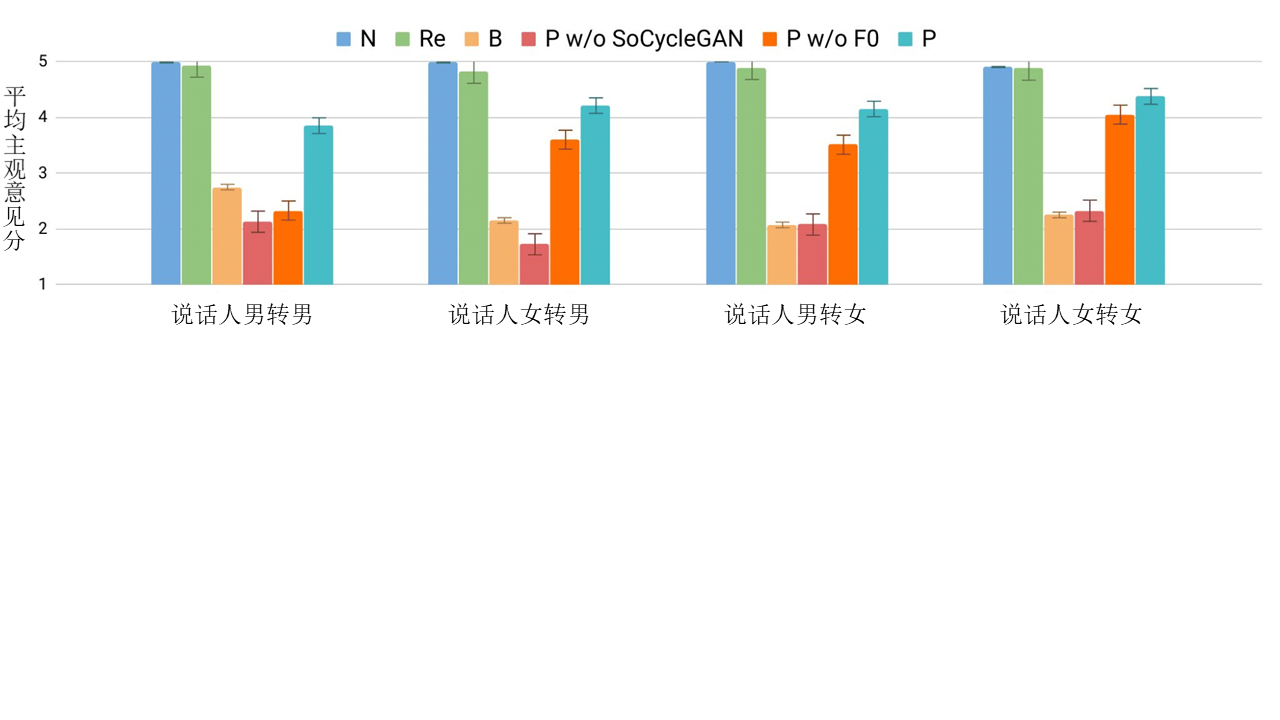
\includegraphics[width=13cm,trim=0 290 0 0,clip]{figure/4_mos.png}
    \bicaption[不同方法在语音自然度上的平均主观意见分对比图]
    {不同方法在语音自然度上的平均主观意见分对比图}
    {MOS comparison among different methods}
    \label{fig:mos}
\end{figure}

\begin{figure}[!htp]
    \centering
    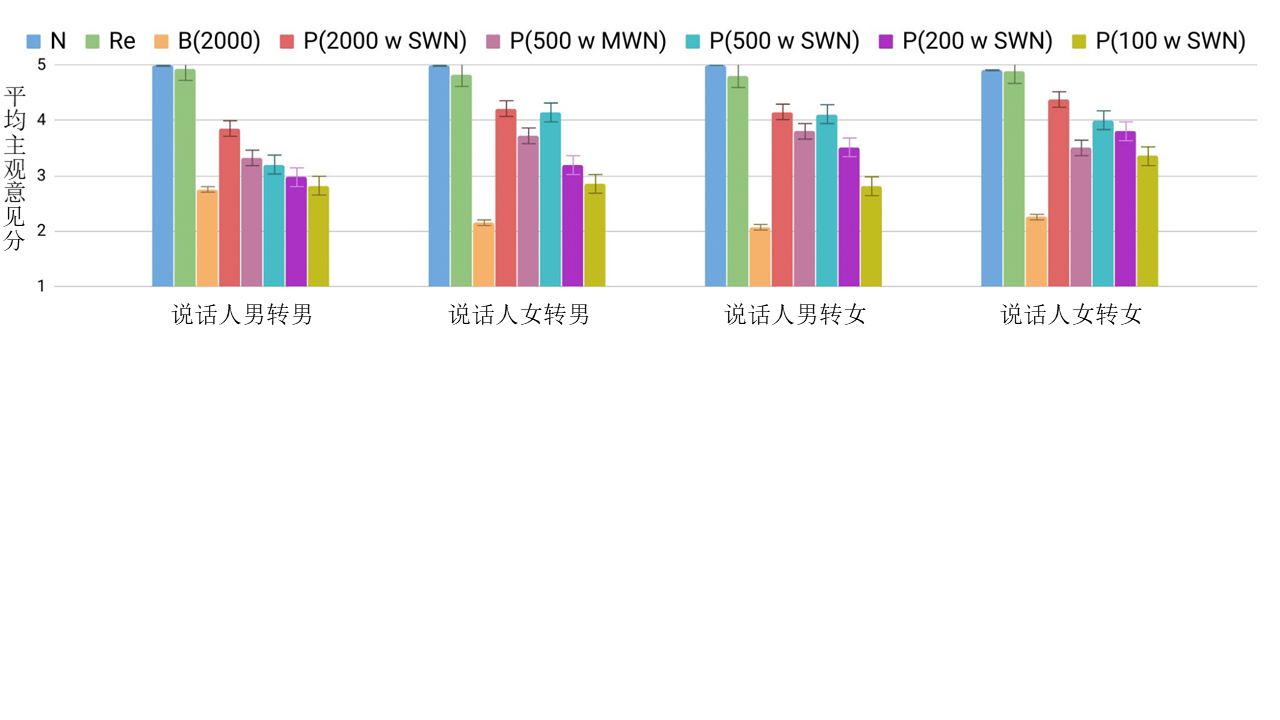
\includegraphics[width=13cm,trim=0 290 0 20,clip]{figure/4_mosdata.png}
    \bicaption[不同大小训练数据集在语音自然度上的平均主观意见分对比图]
    {不同大小训练数据集在语音自然度上的平均主观意见分对比图}
    {MOS comparison among different training data set}
    \label{fig:mosdata}
\end{figure}


图~\ref{fig:mos}展示了MOS测试的结果。对比系统P和P w/o SoCycleGAN,可以看到半优化CycleGAN在自然度上的提升。
从P和P w/o F0的对比,也能发现基频辅助特征的提升,
尤其在男性到男性的实验中(在该实验中音调错误问题最为严重)。
图~\ref{fig:mosdata}展示了所提出系统在不同训练数据量下的性能对比。2000,500,200和100分别代表训练数据集的大小。
SWN代表单说话人WaveNet,是由2000句特定说话人的训练集训练而成,
用以测试半优化CycleGAN的上界。MWN代表多说话人的WaveNet,是由十个中文说话人十几小时数据训练而成。
可以发现提出的系统在至少500句的训练集上可以生成较高音质的转换音频。
注意到我们对于小数据集没有对模型结构进行调整,因此在音质上仍有提升的空间。
相似度实验的结果在图~\ref{fig:sim}展示,可以发现所提出的框架在四个说话人对上都有更好的相似度表现。


\begin{figure}[!htp]
    \centering
    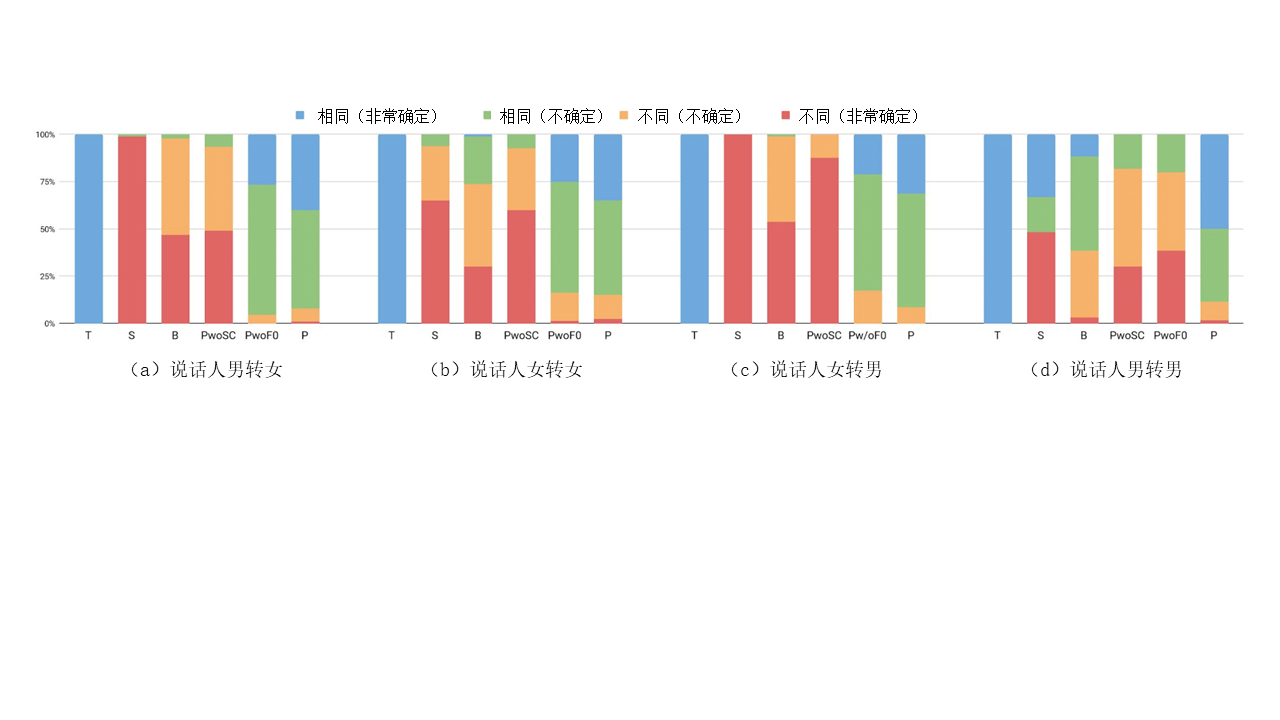
\includegraphics[width=14cm,trim=25 250 40 60,clip]{figure/4_sim.png}
    \bicaption[不同系统在四个说话人对上的相似度对比图]
    {不同系统在四个说话人对上的相似度对比图}
    {Comparison of similarity to target speaker in four speaker pairs}
    \label{fig:sim}
\end{figure}

\section{本章小结}

本章介绍了一种高音质的非平行语音转换框架,针对标准CycleGAN-VC存在的两个问题,
本章提出半优化CycleGAN和基频辅助特征,
并说明了这两个结构可以在基于梅尔频谱的WaveNet声码器下生成高音质的转换语音。
对比标准CycleGAN,半优化CycleGAN对语音自然度和相似度有着较为明显的提升。
基频辅助特征的引入同样也帮助模型更好地从梅尔频谱中学习到基频信息的表示和转换。
主观评测和客观评测表示,
所提出的系统表现优于标准CycleGAN和WORLD声码器的系统和标准CycleGAN和WaveNet声码器的系统。
下一章将介绍该框架在难度更大的语音转换任务:跨语种转换任务上的优化。

